\documentclass[]{article}
\usepackage{lmodern}
\usepackage{amssymb,amsmath}
\usepackage{ifxetex,ifluatex}
\usepackage{fixltx2e} % provides \textsubscript
\ifnum 0\ifxetex 1\fi\ifluatex 1\fi=0 % if pdftex
  \usepackage[T1]{fontenc}
  \usepackage[utf8]{inputenc}
\else % if luatex or xelatex
  \ifxetex
    \usepackage{mathspec}
    \usepackage{xltxtra,xunicode}
  \else
    \usepackage{fontspec}
  \fi
  \defaultfontfeatures{Mapping=tex-text,Scale=MatchLowercase}
  \newcommand{\euro}{€}
\fi
% use upquote if available, for straight quotes in verbatim environments
\IfFileExists{upquote.sty}{\usepackage{upquote}}{}
% use microtype if available
\IfFileExists{microtype.sty}{\usepackage{microtype}}{}
\usepackage[margin=1in]{geometry}
\usepackage{color}
\usepackage{fancyvrb}
\newcommand{\VerbBar}{|}
\newcommand{\VERB}{\Verb[commandchars=\\\{\}]}
\DefineVerbatimEnvironment{Highlighting}{Verbatim}{commandchars=\\\{\}}
% Add ',fontsize=\small' for more characters per line
\newenvironment{Shaded}{}{}
\newcommand{\AlertTok}[1]{\textcolor[rgb]{1.00,0.00,0.00}{\textbf{#1}}}
\newcommand{\AnnotationTok}[1]{\textcolor[rgb]{0.38,0.63,0.69}{\textbf{\textit{#1}}}}
\newcommand{\AttributeTok}[1]{\textcolor[rgb]{0.49,0.56,0.16}{#1}}
\newcommand{\BaseNTok}[1]{\textcolor[rgb]{0.25,0.63,0.44}{#1}}
\newcommand{\BuiltInTok}[1]{#1}
\newcommand{\CharTok}[1]{\textcolor[rgb]{0.25,0.44,0.63}{#1}}
\newcommand{\CommentTok}[1]{\textcolor[rgb]{0.38,0.63,0.69}{\textit{#1}}}
\newcommand{\CommentVarTok}[1]{\textcolor[rgb]{0.38,0.63,0.69}{\textbf{\textit{#1}}}}
\newcommand{\ConstantTok}[1]{\textcolor[rgb]{0.53,0.00,0.00}{#1}}
\newcommand{\ControlFlowTok}[1]{\textcolor[rgb]{0.00,0.44,0.13}{\textbf{#1}}}
\newcommand{\DataTypeTok}[1]{\textcolor[rgb]{0.56,0.13,0.00}{#1}}
\newcommand{\DecValTok}[1]{\textcolor[rgb]{0.25,0.63,0.44}{#1}}
\newcommand{\DocumentationTok}[1]{\textcolor[rgb]{0.73,0.13,0.13}{\textit{#1}}}
\newcommand{\ErrorTok}[1]{\textcolor[rgb]{1.00,0.00,0.00}{\textbf{#1}}}
\newcommand{\ExtensionTok}[1]{#1}
\newcommand{\FloatTok}[1]{\textcolor[rgb]{0.25,0.63,0.44}{#1}}
\newcommand{\FunctionTok}[1]{\textcolor[rgb]{0.02,0.16,0.49}{#1}}
\newcommand{\ImportTok}[1]{#1}
\newcommand{\InformationTok}[1]{\textcolor[rgb]{0.38,0.63,0.69}{\textbf{\textit{#1}}}}
\newcommand{\KeywordTok}[1]{\textcolor[rgb]{0.00,0.44,0.13}{\textbf{#1}}}
\newcommand{\NormalTok}[1]{#1}
\newcommand{\OperatorTok}[1]{\textcolor[rgb]{0.40,0.40,0.40}{#1}}
\newcommand{\OtherTok}[1]{\textcolor[rgb]{0.00,0.44,0.13}{#1}}
\newcommand{\PreprocessorTok}[1]{\textcolor[rgb]{0.74,0.48,0.00}{#1}}
\newcommand{\RegionMarkerTok}[1]{#1}
\newcommand{\SpecialCharTok}[1]{\textcolor[rgb]{0.25,0.44,0.63}{#1}}
\newcommand{\SpecialStringTok}[1]{\textcolor[rgb]{0.73,0.40,0.53}{#1}}
\newcommand{\StringTok}[1]{\textcolor[rgb]{0.25,0.44,0.63}{#1}}
\newcommand{\VariableTok}[1]{\textcolor[rgb]{0.10,0.09,0.49}{#1}}
\newcommand{\VerbatimStringTok}[1]{\textcolor[rgb]{0.25,0.44,0.63}{#1}}
\newcommand{\WarningTok}[1]{\textcolor[rgb]{0.38,0.63,0.69}{\textbf{\textit{#1}}}}
\usepackage{graphicx}
\makeatletter
\def\maxwidth{\ifdim\Gin@nat@width>\linewidth\linewidth\else\Gin@nat@width\fi}
\def\maxheight{\ifdim\Gin@nat@height>\textheight\textheight\else\Gin@nat@height\fi}
\makeatother
% Scale images if necessary, so that they will not overflow the page
% margins by default, and it is still possible to overwrite the defaults
% using explicit options in \includegraphics[width, height, ...]{}
\setkeys{Gin}{width=\maxwidth,height=\maxheight,keepaspectratio}
\ifxetex
  \usepackage[setpagesize=false, % page size defined by xetex
              unicode=false, % unicode breaks when used with xetex
              xetex]{hyperref}
\else
  \usepackage[unicode=true]{hyperref}
\fi
\hypersetup{breaklinks=true,
            bookmarks=true,
            pdfauthor={Justin Le},
            pdftitle={Tries with Recursion Schemes},
            colorlinks=true,
            citecolor=blue,
            urlcolor=blue,
            linkcolor=magenta,
            pdfborder={0 0 0}}
\urlstyle{same}  % don't use monospace font for urls
% Make links footnotes instead of hotlinks:
\renewcommand{\href}[2]{#2\footnote{\url{#1}}}
\setlength{\parindent}{0pt}
\setlength{\parskip}{6pt plus 2pt minus 1pt}
\setlength{\emergencystretch}{3em}  % prevent overfull lines
\setcounter{secnumdepth}{0}

\title{Tries with Recursion Schemes}
\author{Justin Le}

\begin{document}
\maketitle

\emph{Originally posted on
\textbf{\href{https://blog.jle.im/entry/tries-with-recursion-schemes.html}{in
Code}}.}

Not too long ago, I was browsing the
\href{https://www.reddit.com/r/PrequelMemes}{prequel memes subreddit} --- a
community built around creative ways of remixing and re-contextualizing quotes
from the cinematic corpus of the three Star Wars prequel movies --- when I
noticed that a fad was in progress
\href{https://www.reddit.com/r/PrequelMemes/comments/9w59t4/i_expanded_it/}{constructing
tries based on quotes as keys} indexing stills from the movie corresponding to
those quotes.

This inspired me to try playing around with some tries myself, and it gave me an
excuse to play around with
\emph{\href{https://hackage.haskell.org/package/recursion-schemes}{recursion-schemes}}
(one of my favorite Haskell libraries). If you haven't heard about it yet,
\emph{recursion-schemes} (and the similar library
\emph{\href{https://hackage.haskell.org/package/data-fix}{data-fix}}) abstracts
over common recursive functions written on recursive data types. It exploits the
fact that a lot of recursive functions for different recursive data types all
really follow the same pattern and gives us powerful tools for writing cleaner
and safer code, and also for seeing our data types in a different light. The
library is a pathway to many viewpoints --- some considered to be particularly
natural.

Recursion schemes is a perfect example of those amazing accidents that happen
throughout the Haskell ecosystem: an extremely ``theoretically beautiful''
abstraction that also happens to be extremely useful for writing industrially
rigorous code.

Is it possible to learn this power? Yes! As a fun intermediate-level Haskell
project, let's build a trie data type in Haskell based on
\emph{recursion-schemes} to see what it has to offer!

\hypertarget{its-trie-then}{%
\section{It's Trie, Then}\label{its-trie-then}}

A \href{https://en.wikipedia.org/wiki/Trie}{trie} (prefix tree) is a classic
example of a simple yet powerful data type most people first encounter in
college courses (I remember being introduced to it through a project
implementing a boggle solver). The name comes from a pun on the word
``re-\emph{trie}-val''.

Wikipedia has a nice picture:

\begin{figure}
\centering
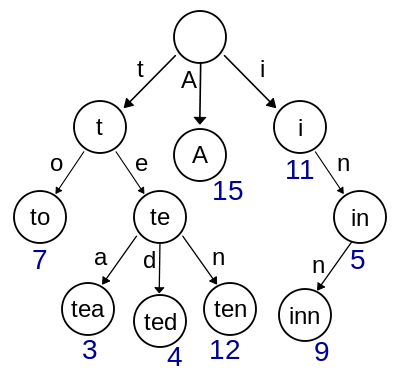
\includegraphics{/img/entries/trie/wiki-trie.png}
\caption{Sample Trie from Wikipedia, indexing lists of Char to Ints}
\end{figure}

API-wise, it is very similar to an \emph{associative map}, like the \texttt{Map}
type from
\emph{\href{https://hackage.haskell.org/package/containers/docs/Data-Map-Lazy.html}{containers}}.
It stores ``keys'' to ``values'', and you can insert a value at a given key,
lookup the value stored at a given key, or delete the value at a given key.
However, it is designed to be easy to (iteratively) find keys matching a given
\emph{prefix}. It's also really fast to check if a given key is \emph{not} in
the trie, since it can return \texttt{False} as soon as a prefix is not found
anywhere in the trie.

The main difference is in implementation: the keys are \emph{strings of tokens},
and it is internally represented as a multi-level tree: if your keys are words,
then the first level is the first letter, the second level is the letter, etc.
In the example above, the trie stores the keys \texttt{to}, \texttt{tea},
\texttt{ted}, \texttt{ten}, \texttt{A}, \texttt{i}, \texttt{in}, and
\texttt{inn} to the values 7, 3, 4, 12, 15, 11, 5, and 9, respectively. As we
see, it is possible for one key to completely overlap another (like \texttt{in}
storing 5, and \texttt{inn} storing 9). We can also have \emph{partial} overlaps
(like \texttt{tea}, storing 3, and \texttt{ted} storing 4), whose common prefix
(\texttt{te}) has no value stored under it.

\hypertarget{haskell-tries}{%
\section{Haskell Tries}\label{haskell-tries}}

We can represent this in Haskell by representing each layer as a \texttt{Map} of
a token to the next layer of subtries.

\begin{Shaded}
\begin{Highlighting}[]
\CommentTok{-- source: https://github.com/mstksg/inCode/tree/master/code-samples/trie/trie.hs#L32-L33}

\KeywordTok{data} \DataTypeTok{Trie}\NormalTok{  k v   }\FunctionTok{=} \DataTypeTok{MkT}\NormalTok{  (}\DataTypeTok{Maybe}\NormalTok{ v) (}\DataTypeTok{Map}\NormalTok{ k (}\DataTypeTok{Trie}\NormalTok{ k v))}
  \KeywordTok{deriving} \DataTypeTok{Show}
\end{Highlighting}
\end{Shaded}

A \texttt{Trie\ k\ v} will have keys of type \texttt{{[}k{]}}, where \texttt{k}
is the key token type, and values of type \texttt{v}. Each layer might have a
value (\texttt{Maybe\ v}), and branches out to each new layer.

We could write the trie storing \texttt{(to,\ 9)}, \texttt{(ton,\ 3)}, and
\texttt{(tax,\ 2)} as:

\begin{Shaded}
\begin{Highlighting}[]
\CommentTok{-- source: https://github.com/mstksg/inCode/tree/master/code-samples/trie/trie.hs#L48-L61}

\OtherTok{testTrie ::} \DataTypeTok{Trie} \DataTypeTok{Char} \DataTypeTok{Int}
\NormalTok{testTrie }\FunctionTok{=} \DataTypeTok{MkT} \DataTypeTok{Nothing} \FunctionTok{$}\NormalTok{ M.fromList [}
\NormalTok{      (}\CharTok{'t'}\NormalTok{, }\DataTypeTok{MkT} \DataTypeTok{Nothing} \FunctionTok{$}\NormalTok{ M.fromList [}
\NormalTok{          (}\CharTok{'o'}\NormalTok{, }\DataTypeTok{MkT}\NormalTok{ (}\DataTypeTok{Just} \DecValTok{9}\NormalTok{) }\FunctionTok{$}\NormalTok{ M.fromList [}
\NormalTok{              ( }\CharTok{'n'}\NormalTok{, }\DataTypeTok{MkT}\NormalTok{ (}\DataTypeTok{Just} \DecValTok{3}\NormalTok{) M.empty )}
\NormalTok{            ]}
\NormalTok{          )}
\NormalTok{        , (}\CharTok{'a'}\NormalTok{, }\DataTypeTok{MkT} \DataTypeTok{Nothing} \FunctionTok{$}\NormalTok{ M.fromList [}
\NormalTok{              ( }\CharTok{'x'}\NormalTok{, }\DataTypeTok{MkT}\NormalTok{ (}\DataTypeTok{Just} \DecValTok{2}\NormalTok{) M.empty )}
\NormalTok{            ]}
\NormalTok{          )}
\NormalTok{        ]}
\NormalTok{      )}
\NormalTok{    ]}
\end{Highlighting}
\end{Shaded}

Note that this construction isn't particularly sound, since it's possible to
represent invalid keys that have branches that lead to nothing. This mostly
becomes troublesome when we implement \texttt{delete}, but we won't be worrying
about that for now. In Haskell, we have the choice to be as safe or unsafe as we
want for a given situation. However, a ``correct-by-construction'' trie is in
the next part of this series :)

\hypertarget{recursion-schemes-an-elegant-weapon}{%
\subsection{Recursion Schemes: An Elegant
Weapon}\label{recursion-schemes-an-elegant-weapon}}

Now, \texttt{Trie} as written up there is an \emph{explicitly recursive} data
type. This is common practice, but it's not a particularly ideal situation. The
problem with explicitly recursive data types is that to work with them, you
often rely on explicitly recursive functions.

Explicitly recursive functions are notoriously difficult to write, understand,
and maintain. It's extremely easy to accidentally write an infinite loop, and
explicit recursion is often called ``the GOTO of functional programming''.

However, There's a trick we can use to ``factor out'' the recursion in our data
type. The trick is to replace the recursive occurrence of \texttt{Trie\ a} (in
the \texttt{Cons} constructor) with a ``placeholder'' variable:

\begin{Shaded}
\begin{Highlighting}[]
\CommentTok{-- source: https://github.com/mstksg/inCode/tree/master/code-samples/trie/trie.hs#L32-L36}

\KeywordTok{data} \DataTypeTok{Trie}\NormalTok{  k v   }\FunctionTok{=} \DataTypeTok{MkT}\NormalTok{  (}\DataTypeTok{Maybe}\NormalTok{ v) (}\DataTypeTok{Map}\NormalTok{ k (}\DataTypeTok{Trie}\NormalTok{ k v))}
  \KeywordTok{deriving} \DataTypeTok{Show}

\KeywordTok{data} \DataTypeTok{TrieF}\NormalTok{ k v x }\FunctionTok{=} \DataTypeTok{MkTF}\NormalTok{ (}\DataTypeTok{Maybe}\NormalTok{ v) (}\DataTypeTok{Map}\NormalTok{ k x         )}
  \KeywordTok{deriving}\NormalTok{ (}\DataTypeTok{Functor}\NormalTok{, }\DataTypeTok{Show}\NormalTok{)}
\end{Highlighting}
\end{Shaded}

\texttt{TrieF} represents, essentially, ``one layer'' of a \texttt{Trie}. It
contains all of the \emph{structure} of a single layer of a \texttt{Trie}: it
contains all of the ``guts'' of what makes a trie a trie, \emph{except the
recursion}. It allows us to work with a single layer of a trie, encapsulating
the essential structure. Later on, we'll see that this means we sometimes don't
even need the original (recursive) \texttt{Trie} at all, if all we just care
about is the structure.

We'll use \texttt{TrieF} as a non-recursive ``view'' into a single layer of a
\texttt{Trie}. We can do this because \emph{recursion-schemes} gives combinators
(known as ``recursion schemes'') to abstract over common explicit recursion
patterns. The key to using \emph{recursion-schemes} is recognizing which
combinators abstracts over the type of recursion you're using. It's all about
becoming familiar with the ``zoo'' of (colorfully named) recursion schemes you
can pick from, and identifying which one does the job in your situation.

That's the high-level view --- let's dive into writing out the API of our
\texttt{Trie}!

\hypertarget{coarse-boilerplate}{%
\subsection{Coarse boilerplate}\label{coarse-boilerplate}}

One thing we need to do before we can start: we need to tell
\emph{recursion-schemes} to link \texttt{TrieF} with \texttt{Trie}. In the
nomenclature of \emph{recursion-schemes}, \texttt{TrieF} is known as the ``base
type'', and \texttt{Trie} is called ``the fixed-point''.

Linking them requires some boilerplate, which is basically converting back and
forth from \texttt{Trie} to \texttt{TrieF}.

\begin{Shaded}
\begin{Highlighting}[]
\CommentTok{-- source: https://github.com/mstksg/inCode/tree/master/code-samples/trie/trie.hs#L38-L46}

\KeywordTok{type} \KeywordTok{instance} \DataTypeTok{Base}\NormalTok{ (}\DataTypeTok{Trie}\NormalTok{ k v) }\FunctionTok{=} \DataTypeTok{TrieF}\NormalTok{ k v}

\KeywordTok{instance} \DataTypeTok{Recursive}\NormalTok{ (}\DataTypeTok{Trie}\NormalTok{ k v) }\KeywordTok{where}
\OtherTok{    project ::} \DataTypeTok{Trie}\NormalTok{ k v }\OtherTok{->} \DataTypeTok{TrieF}\NormalTok{ k v (}\DataTypeTok{Trie}\NormalTok{ k v)}
\NormalTok{    project (}\DataTypeTok{MkT}\NormalTok{ v xs) }\FunctionTok{=} \DataTypeTok{MkTF}\NormalTok{ v xs}

\KeywordTok{instance} \DataTypeTok{Corecursive}\NormalTok{ (}\DataTypeTok{Trie}\NormalTok{ k v) }\KeywordTok{where}
\OtherTok{    embed ::} \DataTypeTok{TrieF}\NormalTok{ k v (}\DataTypeTok{Trie}\NormalTok{ k v) }\OtherTok{->} \DataTypeTok{Trie}\NormalTok{ k v}
\NormalTok{    embed (}\DataTypeTok{MkTF}\NormalTok{ v xs) }\FunctionTok{=} \DataTypeTok{MkT}\NormalTok{ v xs}
\end{Highlighting}
\end{Shaded}

Basically we just link the constructors and fields of \texttt{MkT} and
\texttt{MkTF} together.

Like the adolescent Anakin Skywalker, we usually don't like boilerplate. It's
coarse and rough and irritating, and it gets everywhere. As with all
boilerplate, it is sometimes useful to clean it up a bit using Template Haskell.
The \emph{recursion-schemes} library offers such splice:

\begin{Shaded}
\begin{Highlighting}[]
\KeywordTok{data} \DataTypeTok{Trie}\NormalTok{ k v }\FunctionTok{=} \DataTypeTok{MkT}\NormalTok{ (}\DataTypeTok{Maybe}\NormalTok{ v) (}\DataTypeTok{Map}\NormalTok{ k (}\DataTypeTok{Trie}\NormalTok{ k v))}
  \KeywordTok{deriving} \DataTypeTok{Show}

\NormalTok{makeBaseFunctor ''}\DataTypeTok{Trie}
\end{Highlighting}
\end{Shaded}

This will define \texttt{TrieF} with the \texttt{MkTF} constructor, and not just
the \texttt{Base} type family, but the \texttt{Recursive} and
\texttt{Corecursive} instances, too. It might even be more efficient than our
hand-written way.

\hypertarget{humbly-making-our-way-across-the-universe}{%
\section{Humbly making our way across the
universe}\label{humbly-making-our-way-across-the-universe}}

Time to explore the ``zoo'' of recursion schemes a bit! This is where the fun
begins.

Whenever you get a new recursive type and base functor, a good first thing to
try out is testing out \texttt{cata} and \texttt{ana} (catamorphisms and
anamorphisms), the basic ``folder'' and ``unfolder''.

\hypertarget{ill-try-folding-thats-a-good-trick}{%
\subsection{I'll try folding, that's a good
trick!}\label{ill-try-folding-thats-a-good-trick}}

Catamorphisms are functions that ``combine'' or ``fold'' every layer of our
recursive type into a single value. If we want to write a function of type
\texttt{Trie\ k\ v\ -\textgreater{}\ A}, we can reach first for a catamorphism.

Catamorphisms work by folding layer-by-layer, from the bottom up. We can write
one by defining ``what to do with each layer''. This description comes in the
form of an ``algebra'' in terms of the base functor:

\begin{Shaded}
\begin{Highlighting}[]
\OtherTok{myAlg ::} \DataTypeTok{TrieF}\NormalTok{ k v }\DataTypeTok{A} \OtherTok{->} \DataTypeTok{A}
\end{Highlighting}
\end{Shaded}

If we think of \texttt{TrieF\ k\ v\ a} as ``one layer'' of a
\texttt{Trie\ k\ v}, then \texttt{TrieF\ k\ v\ A\ -\textgreater{}\ A} describes
how to fold up one layer of our \texttt{Trie\ k\ v} into our final result value
(here, of type \texttt{A}). Remember that a \texttt{TrieF\ k\ v\ A} contains a
\texttt{Maybe\ v} and a \texttt{Map\ k\ A}. The \texttt{A} we are given (as the
values of the given map) are the results of folding up all of the original
subtries along each key; it's the ``results so far''. The leaves of the map
become the very thing we swore to create.

Then, we use \texttt{cata} to ``fold'' our value along the algebra:

\begin{Shaded}
\begin{Highlighting}[]
\NormalTok{cata}\OtherTok{ myAlg ::} \DataTypeTok{Trie}\NormalTok{ k v }\OtherTok{->} \DataTypeTok{A}
\end{Highlighting}
\end{Shaded}

\texttt{cata} starts from the bottom-most layer, runs \texttt{myAlg} on that,
then goes up a layer, running \texttt{myAlg} on the results, then goes up
another layer, running \texttt{myAlg} on those results, etc., until it reaches
the top layer and runs \texttt{myAlg} again to produce the final result.

For example, we'll write a catamorphism that counts how many values/leaves we
have in our trie as an \texttt{Int}. Since our result is an \texttt{Int}, we
know we want an algebra returning an \texttt{Int}:

\begin{Shaded}
\begin{Highlighting}[]
\OtherTok{countAlg ::} \DataTypeTok{TrieF}\NormalTok{ k v }\DataTypeTok{Int} \OtherTok{->} \DataTypeTok{Int}
\end{Highlighting}
\end{Shaded}

This is the basic structure of an algebra: our final result type (\texttt{Int})
becomes the parameter of \texttt{TrieF\ k\ v} (as \texttt{TrieF\ k\ v\ Int}),
and also the result of our algebra.

Remember that a \texttt{Trie\ k\ v} contains a \texttt{Maybe\ v} and a
\texttt{Map\ k\ (Trie\ k\ v)}, and a \texttt{TrieF\ k\ v\ Int} contains a
\texttt{Maybe\ v} and a \texttt{Map\ k\ Int}. In a \texttt{Trie\ k\ v}, the
\texttt{Map} contains all of the subtries under each branch. For
\texttt{countAlg}, in our \texttt{TrieF\ k\ v\ Int} we are given, the
\texttt{Map} contains the \emph{counts} of each of those original subtries under
each branch.

Basically, our task is ``Given a map of sub-counts, how do we find the total
count?''

With this in mind, we can write \texttt{countAlg}:

\begin{Shaded}
\begin{Highlighting}[]
\CommentTok{-- source: https://github.com/mstksg/inCode/tree/master/code-samples/trie/trie.hs#L66-L71}

\OtherTok{countAlg ::} \DataTypeTok{TrieF}\NormalTok{ k v }\DataTypeTok{Int} \OtherTok{->} \DataTypeTok{Int}
\NormalTok{countAlg (}\DataTypeTok{MkTF}\NormalTok{ v subtrieCounts)}
    \FunctionTok{|}\NormalTok{ isJust v  }\FunctionTok{=} \DecValTok{1} \FunctionTok{+}\NormalTok{ subtrieTotal}
    \FunctionTok{|}\NormalTok{ otherwise }\FunctionTok{=}\NormalTok{ subtrieTotal}
  \KeywordTok{where}
\NormalTok{    subtrieTotal }\FunctionTok{=}\NormalTok{ sum subtrieCounts}
\end{Highlighting}
\end{Shaded}

If \texttt{v} is indeed a leaf (it's \texttt{Just}), then it's one plus the
total counts of all of the subtees (remember, the \texttt{Map\ k\ Int} contains
the counts of all of the original subtries, under each key). Otherwise, it's
just the total counts of all of the original subtries.

Our final \texttt{count} is, then:

\begin{Shaded}
\begin{Highlighting}[]
\CommentTok{-- source: https://github.com/mstksg/inCode/tree/master/code-samples/trie/trie.hs#L63-L64}

\OtherTok{count ::} \DataTypeTok{Trie}\NormalTok{ k v }\OtherTok{->} \DataTypeTok{Int}
\NormalTok{count }\FunctionTok{=}\NormalTok{ cata countAlg}
\end{Highlighting}
\end{Shaded}

\begin{Shaded}
\begin{Highlighting}[]
\NormalTok{ghci}\FunctionTok{>}\NormalTok{ count testTrie}
\DecValTok{3}
\end{Highlighting}
\end{Shaded}

We can do something similar by writing a summer, as well, to sum up all values
inside a trie:

\begin{Shaded}
\begin{Highlighting}[]
\CommentTok{-- source: https://github.com/mstksg/inCode/tree/master/code-samples/trie/trie.hs#L73-L77}

\OtherTok{trieSumAlg ::} \DataTypeTok{Num}\NormalTok{ a }\OtherTok{=>} \DataTypeTok{TrieF}\NormalTok{ k a a }\OtherTok{->}\NormalTok{ a}
\NormalTok{trieSumAlg (}\DataTypeTok{MkTF}\NormalTok{ v subtrieSums) }\FunctionTok{=}\NormalTok{ fromMaybe }\DecValTok{0}\NormalTok{ v }\FunctionTok{+}\NormalTok{ sum subtrieSums}

\OtherTok{trieSum ::} \DataTypeTok{Num}\NormalTok{ a }\OtherTok{=>} \DataTypeTok{Trie}\NormalTok{ k a }\OtherTok{->}\NormalTok{ a}
\NormalTok{trieSum }\FunctionTok{=}\NormalTok{ cata trieSumAlg}
\end{Highlighting}
\end{Shaded}

\begin{Shaded}
\begin{Highlighting}[]
\NormalTok{ghci}\FunctionTok{>}\NormalTok{ trieSum testTrie}
\DecValTok{14}
\end{Highlighting}
\end{Shaded}

In the algebra, the \texttt{subtrieSums\ ::\ Map\ k\ a} contains the sum of all
of the subtries. The algebra therefore just adds up all of the subtrie sums with
the value at that layer. ``Given a map of sub-sums, how do we find a total
sum?''

\hypertarget{down-from-the-high-ground}{%
\subsubsection{Down from the High Ground}\label{down-from-the-high-ground}}

Catamorphisms are naturally ``inside-out'', or ``bottom-up''. However, some
operations are more naturally ``outside-in'', or ``top-down''. One immediate
example is
\texttt{lookup\ ::\ {[}k{]}\ -\textgreater{}\ Trie\ k\ v\ -\textgreater{}\ Maybe\ v},
which is quintessentially ``top-down'': it first descends down the first item in
the \texttt{{[}k{]}}, then the second, then the third, etc. until you reach the
end, and return the \texttt{Maybe\ v} at that layer.

Is that\ldots{}legal?

In this case, we can make it legal by inverting control: instead of folding into
a \texttt{Maybe\ v} directly, fold into a ``looker upper'', a
\texttt{{[}k{]}\ -\textgreater{}\ Maybe\ v}. We generate a ``lookup function''
from the bottom-up, and then run that all in the end on the key we want to look
up.

Our algebra will therefore have type:

\begin{Shaded}
\begin{Highlighting}[]
\NormalTok{lookupperAlg}
\OtherTok{    ::} \DataTypeTok{Ord}\NormalTok{ k}
    \OtherTok{=>} \DataTypeTok{TrieF}\NormalTok{ k v ([k] }\OtherTok{->} \DataTypeTok{Maybe}\NormalTok{ v)}
    \OtherTok{->}\NormalTok{ ([k] }\OtherTok{->} \DataTypeTok{Maybe}\NormalTok{ v)}
\end{Highlighting}
\end{Shaded}

A \texttt{TrieF\ k\ v\ ({[}k{]}\ -\textgreater{}\ Maybe\ v)} contains a
\texttt{Maybe\ v} and a \texttt{Map\ k\ ({[}k{]}\ -\textgreater{}\ Maybe\ v)},
or a map of ``lookuppers''. Indexed at each key is function of how to look up a
given key in the original subtrie.

So, we are tasked with ``how to implement a lookupper, given a map of
sub-lookuppers''.

To do this, we can pattern match on the key we are looking up. If it's
\texttt{{[}{]}}, then we just return the current leaf (if it exists). Otherwise,
if it's \texttt{k:ks}, we can \emph{run the lookupper of the subtrie at key
\texttt{k}}.

\begin{Shaded}
\begin{Highlighting}[]
\CommentTok{-- source: https://github.com/mstksg/inCode/tree/master/code-samples/trie/trie.hs#L87-L102}

\NormalTok{lookupperAlg}
\OtherTok{    ::} \DataTypeTok{Ord}\NormalTok{ k}
    \OtherTok{=>} \DataTypeTok{TrieF}\NormalTok{ k v ([k] }\OtherTok{->} \DataTypeTok{Maybe}\NormalTok{ v)}
    \OtherTok{->}\NormalTok{ ([k] }\OtherTok{->} \DataTypeTok{Maybe}\NormalTok{ v)}
\NormalTok{lookupperAlg (}\DataTypeTok{MkTF}\NormalTok{ v lookuppers) }\FunctionTok{=}\NormalTok{ \textbackslash{}}\KeywordTok{case}
\NormalTok{    []   }\OtherTok{->}\NormalTok{ v}
\NormalTok{    k}\FunctionTok{:}\NormalTok{ks }\OtherTok{->} \KeywordTok{case}\NormalTok{ M.lookup k lookuppers }\KeywordTok{of}
      \DataTypeTok{Nothing}        \OtherTok{->} \DataTypeTok{Nothing}
      \DataTypeTok{Just}\NormalTok{ lookupper }\OtherTok{->}\NormalTok{ lookupper ks}

\NormalTok{lookup}
\OtherTok{    ::} \DataTypeTok{Ord}\NormalTok{ k}
    \OtherTok{=>}\NormalTok{ [k]}
    \OtherTok{->} \DataTypeTok{Trie}\NormalTok{ k v}
    \OtherTok{->} \DataTypeTok{Maybe}\NormalTok{ v}
\NormalTok{lookup ks t }\FunctionTok{=}\NormalTok{ cata lookupperAlg t ks}
\end{Highlighting}
\end{Shaded}

(written using the -XLambdaCase extension, allowing for
\texttt{\textbackslash{}case} syntax)

\begin{Shaded}
\begin{Highlighting}[]
\NormalTok{ghci}\FunctionTok{>}\NormalTok{ lookup }\StringTok{"to"}\NormalTok{ testTrie}
\DataTypeTok{Just} \DecValTok{9}
\NormalTok{ghci}\FunctionTok{>}\NormalTok{ lookup }\StringTok{"ton"}\NormalTok{ testTrie}
\DataTypeTok{Just} \DecValTok{3}
\NormalTok{ghci}\FunctionTok{>}\NormalTok{ lookup }\StringTok{"tone"}\NormalTok{ testTrie}
\DataTypeTok{Nothing}
\end{Highlighting}
\end{Shaded}

Note that because \texttt{Map}s have lazy values by default, we only ever
actually generate ``lookuppers'' for subtries under keys that we eventually
descend on; any other subtries will be ignored (and no lookuppers are ever
generated for them).

In the end, this version has all of the same performance characteristics as the
explicitly recursive one; we're assembling a ``lookupper'' that stops as soon as
it sees either a failed lookup (so it doesn't cause any more evaluation later
on), or stops when it reaches the end of its list.

\hypertarget{i-think-the-system-works}{%
\subsubsection{I Think the System Works}\label{i-think-the-system-works}}

We've now written a couple of non-recursive functions to ``query''
\texttt{Trie}. But what was the point, again? What do we gain over writing
explicit versions to query Trie? Why couldn't we just write:

\begin{Shaded}
\begin{Highlighting}[]
\CommentTok{-- source: https://github.com/mstksg/inCode/tree/master/code-samples/trie/trie.hs#L79-L81}

\OtherTok{trieSumExplicit ::} \DataTypeTok{Num}\NormalTok{ a }\OtherTok{=>} \DataTypeTok{Trie}\NormalTok{ k a }\OtherTok{->}\NormalTok{ a}
\NormalTok{trieSumExplicit (}\DataTypeTok{MkT}\NormalTok{ v subtries) }\FunctionTok{=}
\NormalTok{    fromMaybe }\DecValTok{0}\NormalTok{ v }\FunctionTok{+}\NormalTok{ sum (fmap trieSumExplicit subtries)}
\end{Highlighting}
\end{Shaded}

instead of

\begin{Shaded}
\begin{Highlighting}[]
\CommentTok{-- source: https://github.com/mstksg/inCode/tree/master/code-samples/trie/trie.hs#L83-L85}

\OtherTok{trieSumCata ::} \DataTypeTok{Num}\NormalTok{ a }\OtherTok{=>} \DataTypeTok{Trie}\NormalTok{ k a }\OtherTok{->}\NormalTok{ a}
\NormalTok{trieSumCata }\FunctionTok{=}\NormalTok{ cata }\FunctionTok{$}\NormalTok{ \textbackslash{}(}\DataTypeTok{MkTF}\NormalTok{ v subtrieSums) }\OtherTok{->}
\NormalTok{    fromMaybe }\DecValTok{0}\NormalTok{ v }\FunctionTok{+}\NormalTok{ sum subtrieSums}
\end{Highlighting}
\end{Shaded}

One major reason, like I mentioned before, is to avoid using \emph{explicit
recursion}. It's extremely easy when using explicit recursion to accidentally
write an infinite loop, or to mess up your control flow somehow. It's basically
like using \texttt{GOTO} instead of \texttt{while} or \texttt{for} loops in
imperative languages. \texttt{while} and \texttt{for} loops are meant to
abstract over a common type of looping control flow, and provide a disciplined
structure for them. They also are often much easier to read, because as soon as
you see ``while'' or ``for'', it gives you a hint at programmer intent in ways
that an explicit GOTO might not.

Another major reason is to allow you to separate concerns. Writing
\texttt{trieSumExplicit} forces you to think ``how to fold this entire trie''.
Writing \texttt{trieSumAlg} allows us to just focus on ``how to fold \emph{this
immediate} layer''. You only need to ever focus on the immediate layer you are
trying to sum --- and never the entire trie. \texttt{cata} takes your ``how to
fold this immediate layer'' function and turns it into a function that folds an
entire trie, taking care of the recursive descent for you.

\begin{center}\rule{0.5\linewidth}{\linethickness}\end{center}

\textbf{Aside}

Before we move on, I just wanted to mention that \texttt{cata} is not a magic
function. From the clues above, you might actually be able to implement it
yourself. For our \texttt{Trie}, it's:

\begin{Shaded}
\begin{Highlighting}[]
\CommentTok{-- source: https://github.com/mstksg/inCode/tree/master/code-samples/trie/trie.hs#L104-L105}

\OtherTok{cata' ::}\NormalTok{ (}\DataTypeTok{TrieF}\NormalTok{ k v a }\OtherTok{->}\NormalTok{ a) }\OtherTok{->} \DataTypeTok{Trie}\NormalTok{ k v }\OtherTok{->}\NormalTok{ a}
\NormalTok{cata' alg }\FunctionTok{=}\NormalTok{ alg }\FunctionTok{.}\NormalTok{ fmap (cata' alg) }\FunctionTok{.}\NormalTok{ project}
\end{Highlighting}
\end{Shaded}

First we
\texttt{project\ ::\ Trie\ k\ v\ -\textgreater{}\ TrieF\ k\ v\ (Trie\ k\ v)}, to
``de-recursive'' our type. Then we fmap our entire
\texttt{cata\ alg\ ::\ Trie\ k\ v\ -\textgreater{}\ a}. Then we run the
\texttt{alg\ ::\ TrieF\ k\ v\ a\ -\textgreater{}\ a} on the result. Basically,
it's fmap-collapse-then-collapse.

It might be interesting to note that the implementation of
\texttt{cata\textquotesingle{}} here requires explicit recursion. One of the
purposes of using recursion schemes like \texttt{cata} is to avoid directly
using recursion explicitly, and ``off-loading'' the recursion to one reusable
function. So in a sense, it's ironic: \texttt{cata} can save other functions
from explicit recursion, but not itself.

Or, can it? The reason \texttt{cata\textquotesingle{}} is necessarily recursive
here is that our \texttt{Trie} data type is recursive. However, we can actually
encode \texttt{Trie} using an alternative representation, and it's possible to
write \texttt{cata\textquotesingle{}} in a non-recursive way:

\begin{Shaded}
\begin{Highlighting}[]
\CommentTok{-- source: https://github.com/mstksg/inCode/tree/master/code-samples/trie/trie.hs#L107-L110}

\KeywordTok{newtype} \DataTypeTok{MuTrie}\NormalTok{ k v }\FunctionTok{=} \DataTypeTok{MkMT}\NormalTok{ (forall a}\FunctionTok{.}\NormalTok{ (}\DataTypeTok{TrieF}\NormalTok{ k v a }\OtherTok{->}\NormalTok{ a) }\OtherTok{->}\NormalTok{ a)}

\OtherTok{cataMuTrie ::}\NormalTok{ (}\DataTypeTok{TrieF}\NormalTok{ k v a }\OtherTok{->}\NormalTok{ a) }\OtherTok{->} \DataTypeTok{MuTrie}\NormalTok{ k v }\OtherTok{->}\NormalTok{ a}
\NormalTok{cataMuTrie alg (}\DataTypeTok{MkMT}\NormalTok{ f) }\FunctionTok{=}\NormalTok{ f alg}
\end{Highlighting}
\end{Shaded}

\texttt{Trie\textquotesingle{}} is actually isomorphic to \texttt{Trie}, so
they're the same type (it's actually
\texttt{type\ MuTrie\ k\ v\ =\ Mu\ (TrieF\ k\ v)}, using \texttt{Mu} from
\emph{recursion-schemes}). If you don't believe me,
\href{https://github.com/mstksg/inCode/tree/master/code-samples/trie/trie.hs\#L112-L116}{here's
the isomorphism}. This is actually one way we can encode recursive types in a
language that doesn't have any, like
\href{https://github.com/sellout/dada/blob/master/Mu/Type}{dhall}.

\begin{center}\rule{0.5\linewidth}{\linethickness}\end{center}

\hypertarget{generating-tries}{%
\subsection{Generating Tries}\label{generating-tries}}

\emph{Anamorphisms}, the dual of catamorphisms, will make another fine addition
to our collection. They are functions that ``generate'' or ``unfold'' a value of
a recursive type, layer-by-layer. If we want to write a function of type
\texttt{A\ -\textgreater{}\ Trie\ k\ v}, we can reach first for an anamorphism.

Anamorphisms work by unfolding ``layer-by-layer'', from the outside-in
(top-down). We write one by defining ``how to generate the next layer''. This
description comes in the form of a ``coalgebra'' (pronounced like
``co-algebra'', and not like coal energy ``coal-gebra''), in terms of the base
functor:

\begin{Shaded}
\begin{Highlighting}[]
\OtherTok{myCoalg ::} \DataTypeTok{A} \OtherTok{->} \DataTypeTok{TrieF}\NormalTok{ k v }\DataTypeTok{A}
\end{Highlighting}
\end{Shaded}

If we think of \texttt{TrieF\ k\ v\ a} as ``one layer'' of a
\texttt{Trie\ k\ v}, then \texttt{A\ -\textgreater{}\ TrieF\ k\ v\ A} describes
how to generate a new nested layer of our \texttt{Trie\ k\ v} from our initial
``seed'' (here, of type \texttt{A}). It tells us how to generate the next
immediate layer. Remember that a \texttt{TrieF\ k\ v\ A} contains a
\texttt{Maybe\ v} and a \texttt{Map\ k\ A}. The \texttt{A} (the values of the
map) are then used to seed the \emph{new} subtries. The \texttt{A}s in the map
are the ``continue expanding with\ldots{}'' values.

We can then use \texttt{ana} to ``unfold'' our value along the coalgebra:

\begin{Shaded}
\begin{Highlighting}[]
\NormalTok{ana}\OtherTok{ myCoalg ::} \DataTypeTok{A} \OtherTok{->} \DataTypeTok{Trie}\NormalTok{ k v}
\end{Highlighting}
\end{Shaded}

\texttt{ana} starts from an initial seed \texttt{A}, runs \texttt{myCoalg} on
that, and then goes down a layer, running \texttt{myCoalg} on each value in the
map to create new layers, etc., forever and ever. In practice, it usually stops
when we return a \texttt{TrieF} with an empty map, since there are no more seeds
to expand down. However, it's nice to remember we don't have to special-case
this behavior: it arises naturally from the structure of maps.

While I don't have a concrete ``universal'' example (like how we had
\texttt{count} and \texttt{sum} for \texttt{cata}), the general idea is that if
you want to create a value by repeatedly ``expanding leaves'', an anamorphism is
a perfect fit.

An example here that fits well with the nature of a trie is to produce a
``singleton trie'': a trie that has only a single value at a single token string
key.

\begin{Shaded}
\begin{Highlighting}[]
\CommentTok{-- source: https://github.com/mstksg/inCode/tree/master/code-samples/trie/trie.hs#L121-L125}

\OtherTok{mkSingletonCoalg ::}\NormalTok{ v }\OtherTok{->}\NormalTok{ ([k] }\OtherTok{->} \DataTypeTok{TrieF}\NormalTok{ k v [k])}
\NormalTok{mkSingletonCoalg v }\FunctionTok{=}\NormalTok{ singletonCoalg}
  \KeywordTok{where}
\NormalTok{    singletonCoalg []     }\FunctionTok{=} \DataTypeTok{MkTF}\NormalTok{ (}\DataTypeTok{Just}\NormalTok{ v) M.empty}
\NormalTok{    singletonCoalg (k}\FunctionTok{:}\NormalTok{ks) }\FunctionTok{=} \DataTypeTok{MkTF} \DataTypeTok{Nothing}\NormalTok{  (M.singleton k ks)}
\end{Highlighting}
\end{Shaded}

Given a \texttt{v} value, we'll make a coalgebra
\texttt{{[}k{]}\ -\textgreater{}\ TrieF\ k\ v\ {[}k{]}}. Our ``seed'' will be
the \texttt{{[}k{]}} key (token string) we want to insert, and we'll generate
our singleton key by making sub-maps with sub-keys.

Our coalgebra (``layer generating function'') goes like this:

\begin{enumerate}
\def\labelenumi{\arabic{enumi}.}
\item
  If our key-to-insert is empty \texttt{{[}{]}}, then we're here! We're at
  \emph{the layer} where we want to insert the value at, so
  \texttt{MkTF\ (Just\ v)\ M.empty}. Returning \texttt{M.empty} means that we
  don't want to expand anymore, since there are no new seeds to expand into
  subtries.
\item
  If our key-to-insert is \emph{not} empty, then we're \emph{not} here! We
  return \texttt{MkTF\ Nothing}\ldots{}but we know we leave a singleton map
  \texttt{M.singleton\ k\ ks\ ::\ Map\ k\ {[}k{]}} leaving a single seed. When
  we run our coalgebra with \texttt{ana}, \texttt{ana} will go down and expand
  out that single seed (with our coalgebra) into an entire new sub-trie, with
  \texttt{ks} as its seed.
\end{enumerate}

So, we have \texttt{singleton}:

\begin{Shaded}
\begin{Highlighting}[]
\CommentTok{-- source: https://github.com/mstksg/inCode/tree/master/code-samples/trie/trie.hs#L118-L119}

\OtherTok{singleton ::}\NormalTok{ [k] }\OtherTok{->}\NormalTok{ v }\OtherTok{->} \DataTypeTok{Trie}\NormalTok{ k v}
\NormalTok{singleton k v }\FunctionTok{=}\NormalTok{ ana (mkSingletonCoalg v) k}
\end{Highlighting}
\end{Shaded}

We run the coalgebra on our initial seed (the key), and ana will run
\texttt{singletonCoalg} repeatedly, expanding out all of the seeds we deposit,
forever and ever (or at least until there are no more values of the seed type
left, which happens if we return an empty map).

\begin{Shaded}
\begin{Highlighting}[]
\NormalTok{ghci}\FunctionTok{>}\NormalTok{ singleton }\StringTok{"hi"} \DecValTok{7}
\DataTypeTok{MkT} \DataTypeTok{Nothing} \FunctionTok{$}\NormalTok{ M.fromList [}
\NormalTok{    (}\CharTok{'h'}\NormalTok{, }\DataTypeTok{MkT} \DataTypeTok{Nothing} \FunctionTok{$}\NormalTok{ M.fromList [}
\NormalTok{        (}\CharTok{'i'}\NormalTok{, }\DataTypeTok{MkT}\NormalTok{ (}\DataTypeTok{Just} \DecValTok{7}\NormalTok{) M.empty )}
\NormalTok{      ]}
\NormalTok{    )}
\NormalTok{  ]}
\end{Highlighting}
\end{Shaded}

\hypertarget{a-pathway-to-many-subtries}{%
\subsection{A pathway to many subtries}\label{a-pathway-to-many-subtries}}

Now that we've got the basics, let's look at a more interesting anamorphism,
where we leave multiple ``seeds'' along many different keys in the map, to
generate many different subtries from our root. Twice the seeds, double the
subtries.

Let's write a function to generate a \texttt{Trie\ k\ v} from a
\texttt{Map\ {[}k{]}\ v}: Given a map of keys (as token strings), generate a
prefix trie containing every key-value pair in the map.

This might sound complicated, but let's remember the philosophy and approach of
writing an anamorphism: ``How do I generate \emph{one layer}''?

Our \texttt{fromMapCoalg} will take a \texttt{Map\ {[}k{]}\ v} and generate
\texttt{TrieF\ k\ v\ (Map\ {[}k{]}\ v)}: \emph{one single layer} of our new Trie
(in particular, the \emph{top layer}). The values in each of the resultant maps
will be later then watered and expanded into their own fully mature subtries.

So, how do we generate the \emph{top layer} of a prefix trie from a map? Well,
remember, to make a \texttt{TrieF\ k\ v\ (Map\ {[}k{]}\ v)}, we need a
\texttt{Maybe\ v} (the value at this layer) and a
\texttt{Map\ k\ (Map\ {[}k{]}\ v)} (the map of seeds that will each expand into
full subtries).

\begin{itemize}
\tightlist
\item
  If the map contains \texttt{{[}{]}} (the empty string), then there \emph{is a
  value} at this layer. We will return \texttt{Just}.
\item
  In the \texttt{Map\ k\ (Map\ {[}k{]}\ v)}, the value at key \texttt{k} is a
  \texttt{Map} containing all of the key-value pairs in the original map that
  \emph{start with k}.
\end{itemize}

For a concrete example, if we start with
\texttt{M.fromList\ {[}("to",\ 9),\ ("ton",\ 3),\ ("tax",\ 2){]}}, then we want
\texttt{fromMapCoalg} to produce:

\begin{Shaded}
\begin{Highlighting}[]
\NormalTok{fromMap (M.fromList [(}\StringTok{"to"}\NormalTok{, }\DecValTok{9}\NormalTok{), (}\StringTok{"ton"}\NormalTok{, }\DecValTok{3}\NormalTok{), (}\StringTok{"tax"}\NormalTok{, }\DecValTok{2}\NormalTok{)])}
    \FunctionTok{=} \DataTypeTok{MkTF} \DataTypeTok{Nothing}\NormalTok{ (}
\NormalTok{          M.fromList [}
\NormalTok{            (}\CharTok{'t'}\NormalTok{, M.fromList [}
\NormalTok{                (}\StringTok{"o"}\NormalTok{ , }\DecValTok{9}\NormalTok{)}
\NormalTok{              , (}\StringTok{"on"}\NormalTok{, }\DecValTok{3}\NormalTok{)}
\NormalTok{              , (}\StringTok{"ax"}\NormalTok{, }\DecValTok{2}\NormalTok{)}
\NormalTok{              ]}
\NormalTok{            )}
\NormalTok{          ]}
\NormalTok{        )}
\end{Highlighting}
\end{Shaded}

The value is \texttt{Nothing} because we don't have the empty string (so there
is no to-level value), and the map at \texttt{t} contains all of the original
key-value pairs that began with \texttt{t}.

Now that we have the concept, we can implement it using \texttt{Data.Map}
combinators like \texttt{M.lookup}, \texttt{M.toList}, \texttt{M.fromListWith},
and \texttt{M.union}.

\begin{Shaded}
\begin{Highlighting}[]
\CommentTok{-- source: https://github.com/mstksg/inCode/tree/master/code-samples/trie/trie.hs#L127-L142}

\NormalTok{fromMapCoalg}
\OtherTok{    ::} \DataTypeTok{Ord}\NormalTok{ k}
    \OtherTok{=>} \DataTypeTok{Map}\NormalTok{ [k] v}
    \OtherTok{->} \DataTypeTok{TrieF}\NormalTok{ k v (}\DataTypeTok{Map}\NormalTok{ [k] v)}
\NormalTok{fromMapCoalg mp }\FunctionTok{=} \DataTypeTok{MkTF}\NormalTok{ (M.lookup [] mp)}
\NormalTok{                       (M.fromListWith M.union}
\NormalTok{                          [ (k   , M.singleton ks v)}
                          \FunctionTok{|}\NormalTok{ (k}\FunctionTok{:}\NormalTok{ks, v) }\OtherTok{<-}\NormalTok{ M.toList mp}
\NormalTok{                          ]}
\NormalTok{                       )}

\NormalTok{fromMap}
\OtherTok{    ::} \DataTypeTok{Ord}\NormalTok{ k}
    \OtherTok{=>} \DataTypeTok{Map}\NormalTok{ [k] v}
    \OtherTok{->} \DataTypeTok{Trie}\NormalTok{ k v}
\NormalTok{fromMap }\FunctionTok{=}\NormalTok{ ana fromMapCoalg}
\end{Highlighting}
\end{Shaded}

And just like that, we have a way to turn a \texttt{Map\ {[}k{]}} into a
\texttt{Trie\ k}\ldots{}all just from describing how to make \emph{the top-most
layer}. \texttt{ana} extrapolates the rest!

Again, we can ask what the point of this is: why couldn't we just write it
directly recursively? The answers are the same as before: first, to avoid
potential bugs from explicit recursion. Second, to separate concerns: instead of
thinking about how to generate an entire trie, we only need to be think about
how to generate a single layer. \texttt{ana} reads our mind here, and
extrapolates out the entire trie.

\begin{center}\rule{0.5\linewidth}{\linethickness}\end{center}

\textbf{Aside}

Again, let's take some time to reassure ourselves that \texttt{ana} is not a
magic function. You might have been able to guess how it's implemented: it runs
the coalgebra, and then fmaps re-expansion recursively.

\begin{Shaded}
\begin{Highlighting}[]
\CommentTok{-- source: https://github.com/mstksg/inCode/tree/master/code-samples/trie/trie.hs#L144-L145}

\OtherTok{ana' ::}\NormalTok{ (a }\OtherTok{->} \DataTypeTok{TrieF}\NormalTok{ k v a) }\OtherTok{->}\NormalTok{ a }\OtherTok{->} \DataTypeTok{Trie}\NormalTok{ k v}
\NormalTok{ana' coalg }\FunctionTok{=}\NormalTok{ embed }\FunctionTok{.}\NormalTok{ fmap (ana' coalg) }\FunctionTok{.}\NormalTok{ coalg}
\end{Highlighting}
\end{Shaded}

First, we run the \texttt{coalg\ ::\ a\ -\textgreater{}\ TrieF\ k\ v\ a}, then
we fmap our entire \texttt{ana\ coalg\ ::\ a\ -\textgreater{}\ Trie\ k\ v}, then
we \texttt{embed\ ::\ TrieF\ k\ v\ (Trie\ k\ v)\ -\textgreater{}\ Trie\ k\ v}
back into our recursive type.

And again, because \texttt{Trie} is a recursive data type, \texttt{ana} is also
necessarily one. However, like for \texttt{cata}, we can represent \texttt{Trie}
in a way that allows us to write \texttt{ana} in a non-recursive way:

\begin{Shaded}
\begin{Highlighting}[]
\CommentTok{-- source: https://github.com/mstksg/inCode/tree/master/code-samples/trie/trie.hs#L147-L150}

\KeywordTok{data} \DataTypeTok{NuTrie}\NormalTok{ k v }\FunctionTok{=}\NormalTok{ forall a}\FunctionTok{.} \DataTypeTok{MkNT}\NormalTok{ (a }\OtherTok{->} \DataTypeTok{TrieF}\NormalTok{ k v a) a}

\OtherTok{anaNuTrie ::}\NormalTok{ (a }\OtherTok{->} \DataTypeTok{TrieF}\NormalTok{ k v a) }\OtherTok{->}\NormalTok{ a }\OtherTok{->} \DataTypeTok{NuTrie}\NormalTok{ k v }
\NormalTok{anaNuTrie }\FunctionTok{=} \DataTypeTok{MkNT}
\end{Highlighting}
\end{Shaded}

\texttt{NuTrie\ k\ v} here is \texttt{Nu\ (TrieF\ k\ v)}, from
\emph{recursion-schemes}. \texttt{NuTrie} is also isomorphic to \texttt{Trie}
(as seen by
\href{https://github.com/mstksg/inCode/tree/master/code-samples/trie/trie.hs\#L152-L156}{this
isomorphism}), so they are the same type. We can also use it to represent
recursive data types in a non-recursive language (like
\href{https://github.com/sellout/dada/blob/master/Nu/Type}{dhall}).

\begin{center}\rule{0.5\linewidth}{\linethickness}\end{center}

\hypertarget{ive-been-looking-forward-to-this}{%
\section{I've been looking forward to
this}\label{ive-been-looking-forward-to-this}}

So those are some examples to get our feet wet; now it's time to build our
prequel meme trie! Yipee!

We're going to try to re-create this reference trie:
(\href{/img/entries/trie/reference-trie.png}{full size here})

\begin{figure}
\centering
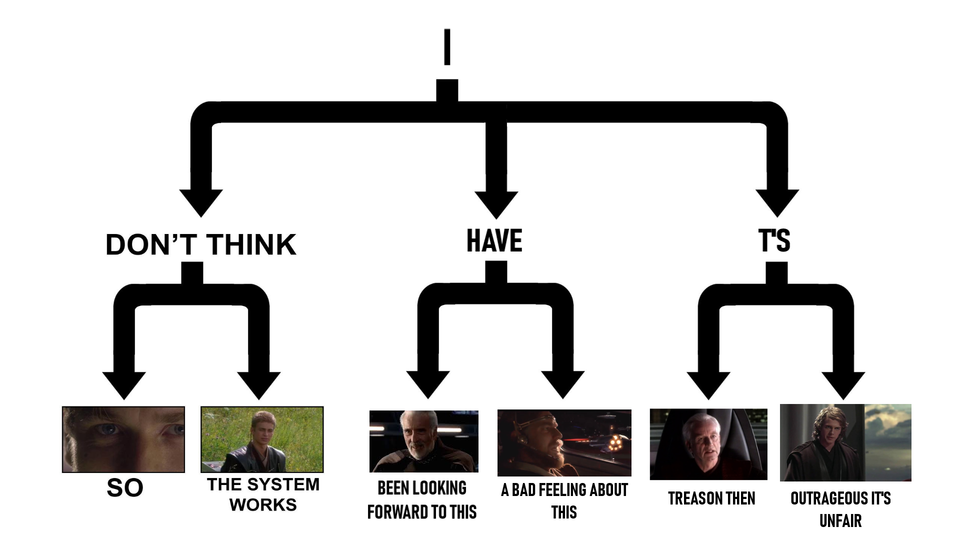
\includegraphics{/img/entries/trie/reference-trie.png}
\caption{Reference trie (credit to
\href{https://www.reddit.com/r/PrequelMemes/comments/9w59t4/i_expanded_it/}{u/Uninventive\_Username})}
\end{figure}

To render our tree, we're going to be using the
\emph{\href{https://hackage.haskell.org/package/graphviz}{graphviz}} library,
which generates a
\emph{\href{https://en.wikipedia.org/wiki/DOT_(graph_description_language)}{DOT
file}} which the \href{https://www.graphviz.org/}{graphviz application} can
render. The \emph{graphviz} library directly renders a value of the graph data
type from \emph{\href{https://hackage.haskell.org/package/fgl}{fgl}}, the
functional graph library that is the de-facto fleshed-out graph manipulation
library of the Haskell ecosystem.

The roadmap seems straightforward:

\begin{enumerate}
\def\labelenumi{\arabic{enumi}.}
\tightlist
\item
  Load our prequel memes into a \texttt{Map\ String\ Label}, a map of quotes to
  their associated macro images (as a \texttt{Label}, which the \emph{graphviz}
  library can render)
\item
  Use \texttt{ana} to turn a \texttt{Map\ String\ Label} into a
  \texttt{Trie\ Char\ Label}
\item
  Use \texttt{cata} to turn a \texttt{Trie\ Char\ Label} into a graph of nodes
  linked by letters, with prequel meme leaves
\item
  Use the \emph{graphviz} library to turn that graph into a DOT file, to be
  rendered by the external graphviz application.
\end{enumerate}

1 and 4 are mainly fumbling around with IO, parsing, and interfacing with
libraries, so 2 and 3 are the interesting steps in our case. We actually already
wrote 2 (in the previous section --- surprise!), so that just leaves 3 to
investigate.

\hypertarget{generating-graphs-is-our-speciality}{%
\subsection{Generating graphs is our
speciality}\label{generating-graphs-is-our-speciality}}

\emph{fgl} provides a two (interchangeable) graph types; for the sake of this
article, we're going to be using \texttt{Gr} from the
\emph{Data.Graph.Inductive.PatriciaTree} module\footnote{Funny story, a
  \href{http://www.drdobbs.com/architecture-and-design/patricia-tries/208800854}{patricia
  tree} is actually itself a variation of trie. In a sense, we are converting a
  trie into a graph represented internally as a trie.}.

The type \texttt{Gr\ a\ b} represents a graph of vertices with labels of type
\texttt{a}, and edges with labels of type \texttt{b}. In our case, for a
\texttt{Trie\ k\ v}, we'll have a graph with nodes of type \texttt{Maybe\ v}
(the leaves, if they exist) and edges of type \texttt{k} (the token linking one
node to the next).

Our end goal, then, is to write a function
\texttt{Trie\ k\ v\ -\textgreater{}\ Gr\ (Maybe\ v)\ k}. Knowing this, we can
jump directly into writing an algebra:

\begin{Shaded}
\begin{Highlighting}[]
\NormalTok{trieGraphAlg}
\OtherTok{    ::} \DataTypeTok{TrieF}\NormalTok{ k v (}\DataTypeTok{Gr}\NormalTok{ (}\DataTypeTok{Maybe}\NormalTok{ v) k)}
    \OtherTok{->} \DataTypeTok{Gr}\NormalTok{ (}\DataTypeTok{Maybe}\NormalTok{ v) k}
\end{Highlighting}
\end{Shaded}

and then using
\texttt{cata\ trieGraphAlg\ ::\ Trie\ k\ v\ -\textgreater{}\ Gr\ (Maybe\ v)\ k}.

This isn't a bad way to go about it, and you won't have \emph{too} many
problems. However, this might be a good learning opportunity to try writing
``monadic'' catamorphisms.

That's because to create a graph using \emph{fgl}, you need to manage Node ID's,
which are represented as \texttt{Int}s. To add a node, you need to generate a
fresh Node ID. \emph{fgl} has some nice tools for managing this, but we can have
some fun by taking care of it ourselves using the so-called ``state monad'',
\texttt{State\ Int}.

We can use \texttt{State\ Int} as a way to generate ``fresh'' node ID's
on-demand, with the action \texttt{fresh}:

\begin{Shaded}
\begin{Highlighting}[]
\CommentTok{-- source: https://github.com/mstksg/inCode/tree/master/code-samples/trie/trie.hs#L158-L159}

\OtherTok{fresh ::} \DataTypeTok{State} \DataTypeTok{Int} \DataTypeTok{Int}
\NormalTok{fresh }\FunctionTok{=}\NormalTok{ state }\FunctionTok{$}\NormalTok{ \textbackslash{}i }\OtherTok{->}\NormalTok{ (i, i}\FunctionTok{+}\DecValTok{1}\NormalTok{)}
\end{Highlighting}
\end{Shaded}

\texttt{fresh} will return the current counter state to produce a new node ID,
and then increment the counter so that the next invocation will return a new
node ID.

In this light, we can frame our big picture as writing a
\texttt{Trie\ k\ v\ -\textgreater{}\ State\ Int\ (Gr\ (Maybe\ v)\ k)}: turn a
\texttt{Trie\ k\ v} into a state action to generate a graph.

To write this, we lay out our algebra:

\begin{Shaded}
\begin{Highlighting}[]
\NormalTok{trieGraphAlg}
\OtherTok{    ::} \DataTypeTok{TrieF}\NormalTok{ k v (}\DataTypeTok{State} \DataTypeTok{Int}\NormalTok{ (}\DataTypeTok{Gr}\NormalTok{ (}\DataTypeTok{Maybe}\NormalTok{ v) k))}
    \OtherTok{->} \DataTypeTok{State} \DataTypeTok{Int}\NormalTok{ (}\DataTypeTok{Gr}\NormalTok{ (}\DataTypeTok{Maybe}\NormalTok{ v) k)}
\end{Highlighting}
\end{Shaded}

We have to write a function ``how to make a state action creating a graph, given
a map of state actions creating sub-graphs''.

One interesting thing to note is that we have a lot to gain from using
``first-class effects'': \texttt{State\ Int\ (Gr\ (Maybe\ v)\ k)} is just a
normal, inert Haskell value that we can manipulate and sequence however we want.
State is not only explicit, but the sequencing of actions (as first-class
values) is also explicit.

We can write this using \emph{fgl} combinators:

\begin{Shaded}
\begin{Highlighting}[]
\CommentTok{-- source: https://github.com/mstksg/inCode/tree/master/code-samples/trie/trie.hs#L166-L177}

\NormalTok{trieGraphAlg}
\OtherTok{    ::} \DataTypeTok{TrieF}\NormalTok{ k v (}\DataTypeTok{State} \DataTypeTok{Int}\NormalTok{ (}\DataTypeTok{Gr}\NormalTok{ (}\DataTypeTok{Maybe}\NormalTok{ v) k))}
    \OtherTok{->} \DataTypeTok{State} \DataTypeTok{Int}\NormalTok{ (}\DataTypeTok{Gr}\NormalTok{ (}\DataTypeTok{Maybe}\NormalTok{ v) k)}
\NormalTok{trieGraphAlg (}\DataTypeTok{MkTF}\NormalTok{ v xs) }\FunctionTok{=} \KeywordTok{do}
\NormalTok{    n         }\OtherTok{<-}\NormalTok{ fresh}
\NormalTok{    subgraphs }\OtherTok{<-}\NormalTok{ sequence xs}
    \CommentTok{--  subbroots :: [(k, Int)]}
    \KeywordTok{let}\NormalTok{ subroots }\FunctionTok{=}\NormalTok{ M.toList }\FunctionTok{.}\NormalTok{ fmap (fst }\FunctionTok{.}\NormalTok{ G.nodeRange) }\FunctionTok{$}\NormalTok{ subgraphs}
\NormalTok{    pure }\FunctionTok{$}\NormalTok{ G.insEdges ((\textbackslash{}(k,i) }\OtherTok{->}\NormalTok{ (n,i,k)) }\FunctionTok{<$>}\NormalTok{ subroots)   }\CommentTok{-- insert root-to-subroots}
         \FunctionTok{.}\NormalTok{ G.insNode (n, v)                     }\CommentTok{-- insert new root}
         \FunctionTok{.}\NormalTok{ M.foldr (G.ufold (}\FunctionTok{G.&}\NormalTok{)) G.empty      }\CommentTok{-- merge all subgraphs}
         \FunctionTok{$}\NormalTok{ subgraphs}
\end{Highlighting}
\end{Shaded}

\begin{enumerate}
\def\labelenumi{\arabic{enumi}.}
\item
  First, generate a fresh node label
\item
  Then, sequence all of the state actions inside the map of sub-graph
  generators. Remember, a
  \texttt{TrieF\ k\ v\ (State\ Int\ (Gr\ (Maybe\ v)\ k))} contains a
  \texttt{Maybe\ v} and a \texttt{Map\ k\ (State\ Int\ (Gr\ (Maybe\ v)\ k))}.
  The map contains State actions to create the sub-graphs, and we use:

\begin{Shaded}
\begin{Highlighting}[]
\NormalTok{sequence}
\OtherTok{    ::} \DataTypeTok{Map}\NormalTok{ k (}\DataTypeTok{State} \DataTypeTok{Int}\NormalTok{ (}\DataTypeTok{Gr}\NormalTok{ (}\DataTypeTok{Maybe}\NormalTok{ v) k))}
    \OtherTok{->} \DataTypeTok{State} \DataTypeTok{Int}\NormalTok{ (}\DataTypeTok{Map}\NormalTok{ k (}\DataTypeTok{Gr}\NormalTok{ (}\DataTypeTok{Maybe}\NormalTok{ v) k))}
\end{Highlighting}
\end{Shaded}

  to turn a map of subgraph-producing actions into an action producing a map of
  subgraphs.

  Note that this is made much simpler because of explicit state sequencing,
  since it gives us the opportunity to choose what ``order'' we want to perform
  our actions. Putting this after \texttt{fresh} ensures that the nodes in the
  subtries all have larger ID's than the root node. If we swap the order of the
  actions, we can actually invert the node ordering.
\item
  Next, it's useful to collect all of the subroots,
  \texttt{subroots\ ::\ {[}(k,\ Int){]}}. These are all of the node id's of the
  roots of each of the subtries, paired with the token leading to that subtrie.
\item
  Now to generate our result:

  \begin{enumerate}
  \def\labelenumii{\alph{enumii}.}
  \tightlist
  \item
    First we merge all subgraphs (using \texttt{G.ufold\ (G.\&)} to merge
    together two graphs)
  \item
    Then, we insert the new root, with our fresh node ID and the new
    \texttt{Maybe\ v} label.
  \item
    Then, we insert all of the edges connecting our new root to the root of all
    our subgraphs (in \texttt{subroots}).
  \end{enumerate}
\end{enumerate}

We can then write our graph generating function using this algebra, and then
running the resulting \texttt{State\ Int\ (Gr\ (Maybe\ v)\ k)} action:

\begin{Shaded}
\begin{Highlighting}[]
\CommentTok{-- source: https://github.com/mstksg/inCode/tree/master/code-samples/trie/trie.hs#L161-L164}

\NormalTok{trieGraph}
\OtherTok{    ::} \DataTypeTok{Trie}\NormalTok{ k v}
    \OtherTok{->} \DataTypeTok{Gr}\NormalTok{ (}\DataTypeTok{Maybe}\NormalTok{ v) k}
\NormalTok{trieGraph }\FunctionTok{=}\NormalTok{ flip evalState }\DecValTok{0} \FunctionTok{.}\NormalTok{ cata trieGraphAlg}
\end{Highlighting}
\end{Shaded}

Finally, we can write our \texttt{mapToGraph}:

\begin{Shaded}
\begin{Highlighting}[]
\NormalTok{mapToGraph}
\OtherTok{    ::} \DataTypeTok{Ord}\NormalTok{ k}
    \OtherTok{=>} \DataTypeTok{Map}\NormalTok{ [k] v}
    \OtherTok{->} \DataTypeTok{Gr}\NormalTok{ (}\DataTypeTok{Maybe}\NormalTok{ v) k}
\NormalTok{mapToGraph }\FunctionTok{=}\NormalTok{ flip evalState }\DecValTok{0}
           \FunctionTok{.}\NormalTok{ cata trieGraphAlg}
           \FunctionTok{.}\NormalTok{ ana fromGraphCoalg}
\end{Highlighting}
\end{Shaded}

\hypertarget{hylomorphisms}{%
\subsection{Hylomorphisms}\label{hylomorphisms}}

Actually, writing things out as \texttt{mapToGraph} gives us some interesting
insight: our function takes a \texttt{Map\ {[}k{]}\ v}, and returns a
\texttt{Gr\ (Maybe\ v)\ k}. Notice that \texttt{Trie\ k\ v} isn't anywhere in
the type signature. This means that, to, the external user, \texttt{Trie}'s role
is completely ``internal''.

In other words, \texttt{Trie} itself doesn't seem to matter at all. We really
want a \texttt{Map\ {[}k{]}\ v\ -\textgreater{}\ Graph\ (Maybe\ v)\ k}, and
we're just using \texttt{Trie} as an \emph{intermediate data structure}. We are
exploiting its structure to do write our full function, and we don't care about
it outside of that. We build it up with \texttt{ana} and then immediately tear
it down with \texttt{cata}, and it is completely invisible to the outside world.

One neat thing about \emph{recursion-schemes} is that it lets us capture this
``the actual fixed-point is only intermediate and is not directly consequential
to the outside world'' pattern. First, we walk ourselves through the following
reasoning steps:

\begin{itemize}
\tightlist
\item
  We don't care about \texttt{Trie} itself as a result our input. We only care
  about it because we exploit its internal structure.
\item
  \texttt{TrieF} \emph{already} expresses the internal structure of
  \texttt{Trie}
\item
  Therefore, if we only want to take advantage of the structure, we really only
  ever need \texttt{TrieF}. We can completely bypass \texttt{Trie}.
\end{itemize}

This should make sense in our case, because the only reason we use \texttt{Trie}
is for its internal structure. But \texttt{TrieF} \emph{already} captures the
internal structure --- thus, we really only need to ever worry about
\texttt{TrieF}. We don't actually care about the recursive data type --- we
never did!

In this spirit, \emph{recursion-schemes} offers the \emph{hylomorphism}
recursion scheme:

\begin{Shaded}
\begin{Highlighting}[]
\NormalTok{hylo}
\OtherTok{    ::}\NormalTok{ (}\DataTypeTok{TrieF}\NormalTok{ k v b }\OtherTok{->}\NormalTok{ b)   }\CommentTok{-- ^ an algebra}
    \OtherTok{->}\NormalTok{ (a }\OtherTok{->} \DataTypeTok{TrieF}\NormalTok{ k v a)   }\CommentTok{-- ^ a coalgebra}
    \OtherTok{->}\NormalTok{ a}
    \OtherTok{->}\NormalTok{ b}
\end{Highlighting}
\end{Shaded}

If we see the coalgebra \texttt{a\ -\textgreater{}\ TrieF\ k\ v\ a} as a
``building'' function, and the algebra
\texttt{TrieF\ k\ v\ b\ -\textgreater{}\ b} as a ``consuming'' function, then
\texttt{hylo} will \emph{build, then immediately consume}. It'll build with the
coalgebra on \texttt{TrieF}, then immediately consume with the algebra on
\texttt{TrieF}. No \texttt{Trie} is ever generated, because it's never
necessary: we're literally just building and immediately consuming
\texttt{TrieF} values.

We could even implement \texttt{hylo} ourselves, to illustrate the ``build and
immediately consume'' property:

\begin{Shaded}
\begin{Highlighting}[]
\CommentTok{-- source: https://github.com/mstksg/inCode/tree/master/code-samples/trie/trie.hs#L185-L192}

\NormalTok{hylo'}
\OtherTok{    ::}\NormalTok{ (}\DataTypeTok{TrieF}\NormalTok{ k v b }\OtherTok{->}\NormalTok{ b)   }\CommentTok{-- ^ an algebra}
    \OtherTok{->}\NormalTok{ (a }\OtherTok{->} \DataTypeTok{TrieF}\NormalTok{ k v a)   }\CommentTok{-- ^ a coalgebra}
    \OtherTok{->}\NormalTok{ a}
    \OtherTok{->}\NormalTok{ b}
\NormalTok{hylo' consume build }\FunctionTok{=}\NormalTok{ consume}
                    \FunctionTok{.}\NormalTok{ fmap (hylo' consume build)}
                    \FunctionTok{.}\NormalTok{ build}
\end{Highlighting}
\end{Shaded}

Note that the implementation of \texttt{hylo} given above works for any
\texttt{Functor} instance: we build and consume along \emph{any}
\texttt{Functor}, taking advantage of the specific functor's structure.

To me, being able to implement a function in terms of \texttt{hylo} (or any
other refolder, like its cousin \texttt{chrono}, the chronomorphism) represents
the ultimate ``victory'' in using \emph{recursion-schemes} to refactor out your
functions. That's because it helps us realize that we never really \emph{cared}
about having a recursive data type in the first place. \texttt{Trie} was never
the actual thing we wanted: we really just wanted its layer-by-layer structure.
This whole time, we just cared about the structure of \texttt{TrieF}, \emph{not}
\texttt{Trie}. Being able to use \texttt{hylo} lets us see that the original
recursive data type was nothing more than a distraction. Through it, we see the
light.

I call the experiencing of making this revelation ``achieving hylomorphism''.

Our final map-to-graph function can therefore be expressed as:

\begin{Shaded}
\begin{Highlighting}[]
\CommentTok{-- source: https://github.com/mstksg/inCode/tree/master/code-samples/trie/trie.hs#L179-L183}

\NormalTok{mapToGraph}
\OtherTok{    ::} \DataTypeTok{Ord}\NormalTok{ k}
    \OtherTok{=>} \DataTypeTok{Map}\NormalTok{ [k] v}
    \OtherTok{->} \DataTypeTok{Gr}\NormalTok{ (}\DataTypeTok{Maybe}\NormalTok{ v) k}
\NormalTok{mapToGraph }\FunctionTok{=}\NormalTok{ flip evalState }\DecValTok{0} \FunctionTok{.}\NormalTok{ hylo trieGraphAlg fromMapCoalg}
\end{Highlighting}
\end{Shaded}

\hypertarget{pack-your-things}{%
\subsection{Pack your things}\label{pack-your-things}}

To wrap things up, I made a text file storing all of the prequel quotes in the
original reference trie along with images stored on my drive: (you can find a
them
\href{https://github.com/mstksg/inCode/tree/master/code-samples/trie/img}{online
here})

\begin{verbatim}
I DON'T THINK SO,img/idts.jpg
I DON'T THINK THE SYSTEM WORKS,img/idttsw.jpg
I HAVE BEEN LOOKING FORWARD TO THIS,img/iblftt.jpg
I HAVE A BAD FEELING ABOUT THIS,img/ihabfat.jpg
IT'S TREASON THEN,img/itt.jpg
IT'S OUTRAGEOUS IT'S UNFAIR,img/tioiu.jpg
\end{verbatim}

We can write a quick parser and aggregator into a
\texttt{Map\ {[}Char{]}\ HTML.Label}, where \texttt{HTML.Label} is from the
\emph{graphviz} library, a renderable object to display on the final image.

\begin{Shaded}
\begin{Highlighting}[]
\CommentTok{-- source: https://github.com/mstksg/inCode/tree/master/code-samples/trie/trie.hs#L194-L203}

\OtherTok{memeMap ::} \DataTypeTok{String} \OtherTok{->} \DataTypeTok{Map} \DataTypeTok{String} \DataTypeTok{HTML.Label}
\NormalTok{memeMap }\FunctionTok{=}\NormalTok{ M.fromList }\FunctionTok{.}\NormalTok{ map (uncurry processLine }\FunctionTok{.}\NormalTok{ span (}\FunctionTok{/=} \CharTok{','}\NormalTok{)) }\FunctionTok{.}\NormalTok{ lines}
  \KeywordTok{where}
\NormalTok{    processLine qt (drop }\DecValTok{1}\OtherTok{->}\NormalTok{img) }\FunctionTok{=}\NormalTok{ (}
\NormalTok{          filter (not }\FunctionTok{.}\NormalTok{ isSpace) qt}
\NormalTok{        , }\DataTypeTok{HTML.Table}\NormalTok{ (}\DataTypeTok{HTML.HTable} \DataTypeTok{Nothing}\NormalTok{ [] [r1,r2])}
\NormalTok{        )}
      \KeywordTok{where}
\NormalTok{        r1 }\FunctionTok{=} \DataTypeTok{HTML.Cells}\NormalTok{ [}\DataTypeTok{HTML.LabelCell}\NormalTok{ [] (}\DataTypeTok{HTML.Text}\NormalTok{ [}\DataTypeTok{HTML.Str}\NormalTok{ (T.pack qt)])]}
\NormalTok{        r2 }\FunctionTok{=} \DataTypeTok{HTML.Cells}\NormalTok{ [}\DataTypeTok{HTML.ImgCell}\NormalTok{   [] (}\DataTypeTok{HTML.Img}\NormalTok{ [}\DataTypeTok{HTML.Src}\NormalTok{ img])]}
\end{Highlighting}
\end{Shaded}

We can also write a small utility function to clean up our final graph; it
deletes nodes that only have one child and compacts them into the node above.
It's just to ``compress'' together strings of nodes that don't have any forks.

\begin{Shaded}
\begin{Highlighting}[]
\CommentTok{-- source: https://github.com/mstksg/inCode/tree/master/code-samples/trie/trie.hs#L226-L236}

\NormalTok{compactify}
\OtherTok{    ::} \DataTypeTok{Gr}\NormalTok{ (}\DataTypeTok{Maybe}\NormalTok{ v) k}
    \OtherTok{->} \DataTypeTok{Gr}\NormalTok{ (}\DataTypeTok{Maybe}\NormalTok{ v) [k]}
\NormalTok{compactify g0 }\FunctionTok{=}\NormalTok{ foldl' go (G.emap (}\FunctionTok{:}\NormalTok{[]) g0) (G.labNodes g0)}
  \KeywordTok{where}
\NormalTok{    go g (i, v) }\FunctionTok{=} \KeywordTok{case}\NormalTok{ (G.inn g i, G.out g i) }\KeywordTok{of}
\NormalTok{      ([(j, _, lj)], [(_, k, lk)])}
        \FunctionTok{|}\NormalTok{ isNothing v }\OtherTok{->}\NormalTok{ G.insEdge (j, k, lj }\FunctionTok{++}\NormalTok{ lk)}
                       \FunctionTok{.}\NormalTok{ G.delNode i }\FunctionTok{.}\NormalTok{ G.delEdges [(j,i),(i,k)]}
                       \FunctionTok{$}\NormalTok{ g}
\NormalTok{      _               }\OtherTok{->}\NormalTok{ g}
\end{Highlighting}
\end{Shaded}

We could have directly outputted a compacted graph from \texttt{graphAlg}, but
for the sake of this post it's a bit cleaner to separate out these concerns.

We'll write a function to turn a \texttt{Gr\ (Maybe\ HTML.Label)\ {[}Char{]}}
into a dot file, using \emph{graphviz} to do most of the work:

\begin{Shaded}
\begin{Highlighting}[]
\CommentTok{-- source: https://github.com/mstksg/inCode/tree/master/code-samples/trie/trie.hs#L205-L215}

\NormalTok{graphDot}
\OtherTok{    ::} \DataTypeTok{Gr}\NormalTok{ (}\DataTypeTok{Maybe} \DataTypeTok{HTML.Label}\NormalTok{) }\DataTypeTok{String}
    \OtherTok{->} \DataTypeTok{T.Text}
\NormalTok{graphDot }\FunctionTok{=}\NormalTok{ GV.printIt }\FunctionTok{.}\NormalTok{ GV.graphToDot params}
  \KeywordTok{where}
\NormalTok{    params }\FunctionTok{=}\NormalTok{ GV.nonClusteredParams}
\NormalTok{      \{ fmtNode }\FunctionTok{=}\NormalTok{ \textbackslash{}(_,  l) }\OtherTok{->} \KeywordTok{case}\NormalTok{ l }\KeywordTok{of}
          \DataTypeTok{Nothing} \OtherTok{->}\NormalTok{ [GV.shape }\DataTypeTok{GV.PointShape}\NormalTok{]}
          \DataTypeTok{Just}\NormalTok{ l' }\OtherTok{->}\NormalTok{ [GV.toLabel l', GV.shape }\DataTypeTok{GV.PlainText}\NormalTok{]}
\NormalTok{      , fmtEdge }\FunctionTok{=}\NormalTok{ \textbackslash{}(_,_,l) }\OtherTok{->}\NormalTok{ [GV.toLabel (concat [}\StringTok{"["}\NormalTok{, l, }\StringTok{"]"}\NormalTok{])]}
\NormalTok{      \}}
\end{Highlighting}
\end{Shaded}

And finally, we can write the entire pipeline:

\begin{Shaded}
\begin{Highlighting}[]
\CommentTok{-- source: https://github.com/mstksg/inCode/tree/master/code-samples/trie/trie.hs#L217-L224}

\NormalTok{memeDot}
\OtherTok{    ::} \DataTypeTok{String}
    \OtherTok{->} \DataTypeTok{T.Text}
\NormalTok{memeDot }\FunctionTok{=}\NormalTok{ graphDot}
        \FunctionTok{.}\NormalTok{ compactify}
        \FunctionTok{.}\NormalTok{ flip evalState }\DecValTok{0}
        \FunctionTok{.}\NormalTok{ hylo trieGraphAlg fromMapCoalg}
        \FunctionTok{.}\NormalTok{ memeMap}
\end{Highlighting}
\end{Shaded}

Shorter than I expected!

This gives us our final result: (\href{/img/entries/trie/meme-trie.png}{full
size here})

\begin{figure}
\centering
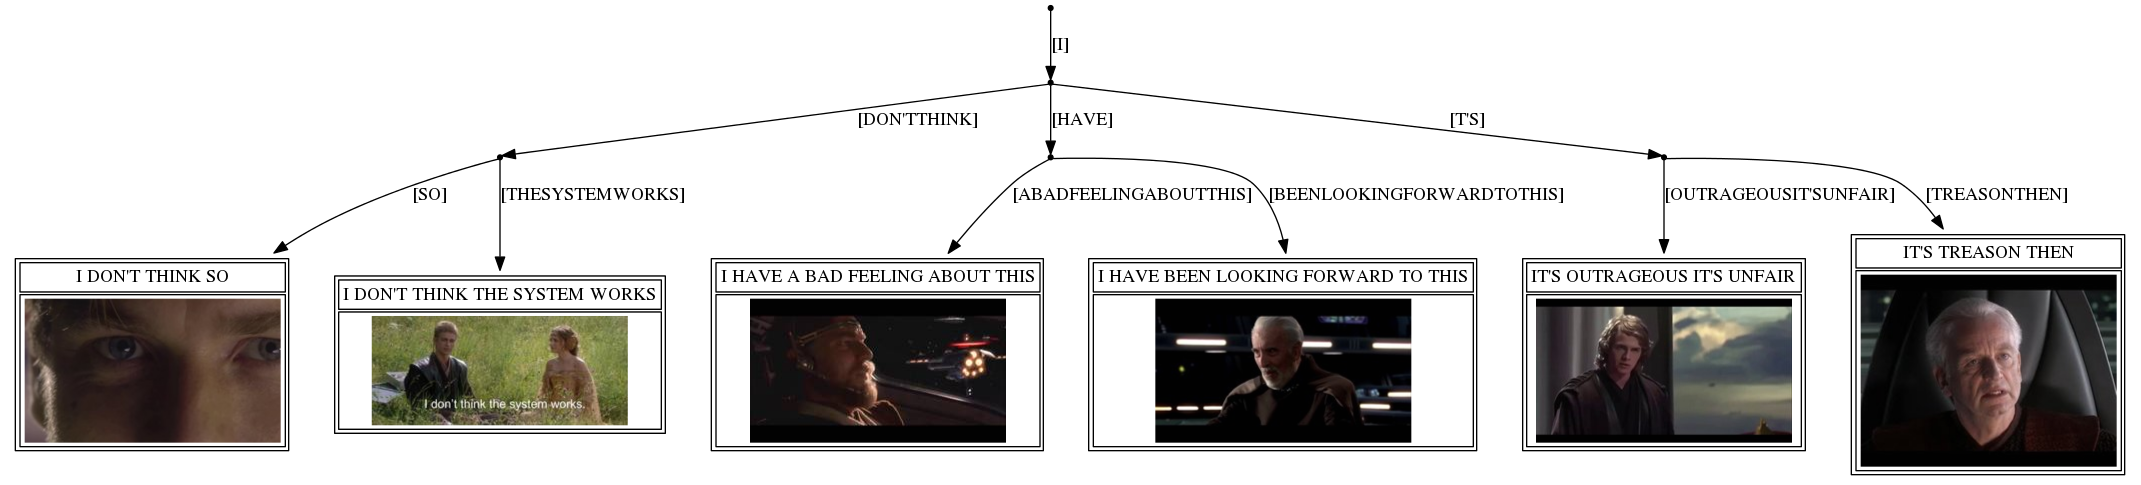
\includegraphics{/img/entries/trie/meme-trie.png}
\caption{Our rendered dotfile, using graphviz}
\end{figure}

There are definitely some things we can tweak with respect to formatting and
position and font sizes and label layouts, but I think this is fairly faithful
to the original structure!

\hypertarget{another-happy-landing}{%
\section{Another happy landing}\label{another-happy-landing}}

There's a lot more we can do with tries, and fleshing out a full interface
allows us to explore a lot of other useful recursion schemes and combinators.

Now that we've familiarized ourselves with a simple tangible example, we're now
free to dive deep. Achieving hylomorphism helps us see past the recursive data
type and directly into the underlying structure of what's going on. And out of
it, we got a pretty helpful meme trie we can show off to our friends.

In the next parts of the series, we'll find out what other viewpoints
\emph{recursion-schemes} has to offer for us!

\hypertarget{signoff}{%
\section{Signoff}\label{signoff}}

Hi, thanks for reading! You can reach me via email at
\href{mailto:justin@jle.im}{\nolinkurl{justin@jle.im}}, or at twitter at
\href{https://twitter.com/mstk}{@mstk}! This post and all others are published
under the \href{https://creativecommons.org/licenses/by-nc-nd/3.0/}{CC-BY-NC-ND
3.0} license. Corrections and edits via pull request are welcome and encouraged
at \href{https://github.com/mstksg/inCode}{the source repository}.

If you feel inclined, or this post was particularly helpful for you, why not
consider \href{https://www.patreon.com/justinle/overview}{supporting me on
Patreon}, or a \href{bitcoin:3D7rmAYgbDnp4gp4rf22THsGt74fNucPDU}{BTC donation}?
:)

\end{document}
